\documentclass{article}
\usepackage{tikz}
\usetikzlibrary{arrows.meta, shapes.geometric, positioning, calc}

\begin{document}

\begin{figure}[h]
  \centering
  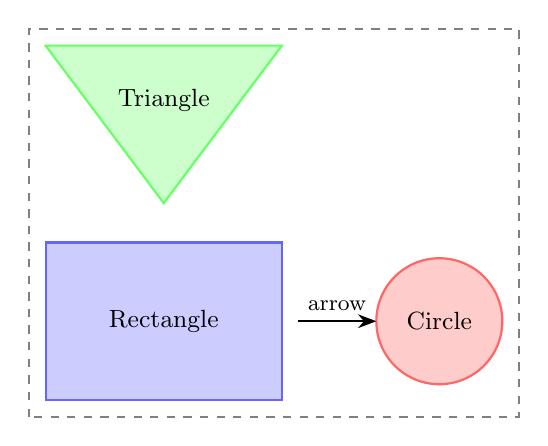
\begin{tikzpicture}[
    % Global options: line width, font size, scale
    line width=0.8pt,
    font=\small,
    scale=1,
  ]
    % --- Filled rectangle ---
    \filldraw[fill=blue!20, draw=blue!60]
      (0,0) rectangle (3,2);
    \node at (1.5,1) {Rectangle};

    % --- Circle with arrow pointing to it ---
    \filldraw[fill=red!20, draw=red!60]
      (5,1) circle (0.8);
    \node at (5,1) {Circle};
    \draw[-{Stealth}] (3.2,1) -- (4.2,1)
      node[midway, above, font=\footnotesize] {arrow};

    % --- Triangle via -- cycle ---
    \filldraw[fill=green!20, draw=green!60]
      (1.5,2.5) -- (0,4.5) -- (3,4.5) -- cycle;
    \node at (1.5,3.8) {Triangle};

    % --- Dashed bounding box around everything (calc library) ---
    \draw[dashed, gray]
      ($(current bounding box.south west)+(-0.2,-0.2)$)
      rectangle
      ($(current bounding box.north east)+(0.2,0.2)$);
  \end{tikzpicture}
  \caption{Basic TikZ 2D shapes.}
  \label{fig:tikz2d}
\end{figure}

\end{document}
